\documentclass[11pt]{article}
\usepackage{deauthor,times,graphicx}

% \usepackage[font=small,labelfont=bf]{caption}
\usepackage{subfig}
\usepackage{wrapfig}
\usepackage{url}

% Note-related commands.
\usepackage{etoolbox}
\usepackage{xcolor}
\usepackage{listings} 
\usepackage{xspace}

\newcommand{\eat}[1]{}
\newcommand{\ys}[1]{\textcolor{blue}{[YS: #1]}}
\newcommand{\mi}[1]{\textcolor{red}{[MI: #1]}}
\newcommand{\as}[1]{\textcolor{green}{[AS: #1]}}
\newcommand{\pretzel}{\textsc{Pretzel}\xspace}
\newcommand{\mlnet}{ML.NET\xspace}
\newcommand{\msft}{Microsoft\xspace}
\newcommand{\at}[1]{\protect\ensuremath{\mathsf{#1}}\xspace}
\newcommand{\stitle}[1]{\noindent{\bf #1}}
\newcommand{\idataview}{\at{DataView}}

\lstdefinelanguage{Scala}{
  keywords={typeof, new, true, false, catch,def,val, function, return, null, catch, switch, var, if, in, while, do, else, case, break},
  keywordstyle=\color{blue}\bfseries,
  ndkeywords={class, export,extends, boolean, throw, implements, import, this, abstract},
  ndkeywordstyle=\color{dkgreen}\bfseries,
  otherkeywords={+, =>,<=, ==, >,< , ||},
  identifierstyle=\color{black},
  sensitive=false,
  comment=[l]{//},
  morecomment=[s]{/*}{*/},
  commentstyle=\color{purple}\ttfamily,
  stringstyle=\color{red}\ttfamily,
  morestring=[b]',
  morestring=[b]",
  moredelim=**[is][\color{red}]{@}{@},
}
\lstset{frame=tb,
  language=Scala,
  aboveskip=3mm,
  belowskip=5mm,
  showstringspaces=false,
  columns=flexible,
  basicstyle={\scriptsize\ttfamily},
  numberstyle=\tiny\color{gray},
  keywordstyle=\color{blue},
  commentstyle=\color{dkgreen},
  stringstyle=\color{mauve},
  breaklines=true,
  breakatwhitespace=true,
  tabsize=3,
  numbers=left,
  xleftmargin=1em,
  framexleftmargin=1em,
}
\lstdefinestyle{fault}{ numbers=none, xleftmargin=1.5em , otherkeywords={ =>,<=, ==, > , ||}}


\begin{document}
\title{From the Edge to the Cloud: Model Serving in ML.NET}
\author{Yunseong Lee, Alberto Scolari, Byung-Gon Chun, Markus Weimer and Matteo Interlandi\\
{\small \{yunseong, bgchun\}@snu.ac.kr, alberto.scolari@polimi.it, \{mweimer, mainterl\}@microsoft.com}}
\maketitle
%\date{Oct 2018} % yule: do we need to write date?

\begin{abstract}
%This is abstract. We are building an awesome system.    
As Machine Learning (ML) is becoming ubiquitously used within applications, developers need effective solutions to build and deploy their ML models across a large set of scenarios, from IoT devices to the cloud.
Unfortunately, the current state of the art in model serving suggests to deliver predictions by running models in containers.
While this solution eases the operationalization of models, we observed that it is not flexible enough to address the variety of ML scenarios encountered in large companies such as Microsoft.  
In this paper, we will overview ML.NET---a recently open sourced ML pipeline framework---and describe how ML models written in ML.NET can be seamlessly integrated into applications.
Finally, we will discuss how model serving can be cast to a database problem, and provide insights on our recent experience in building a database optimizer for ML.NET pipelines. 


\eat{
provide this flexibility and ease, they still lack the ability to optimize the model for the inference phase, which has different characteristics and requirements from the training phase in which the model was built. This is due to those solutions ignoring the actual sequence of operations along the pipeline, treating it only as a black-box. Here, we show the main limitations of this approach and advocate for a white-box approach, where the model structure and state are used to optimize the model itself and manage its resources. Out of these ideas, we built a prototype framework supporting \mlnet models called \pretzel, which shows noticeable improvements in performance and resources usage.}
\end{abstract}

\section{Introduction}
Machine Learning (ML) is transitioning from an art and science into a technology readily available to every developer.
% An effect of this transition is a proliferation of data-driven applications that rely on trained models for functionalities that evade traditional programming due to their complex statistical nature.
In the near future, every application on every platform will rely on trained models for functionalities that evade traditional programming due to their complex statistical nature.
This unfolding future---where most applications make use of at least one model---profoundly differs from the current practice in which data science and software engineering are performed in separate and different processes and sometimes even by different teams and organizations. Furthermore, in current practice, models are routinely deployed and managed in completely distinct ways from other software artifacts: while typical software libraries are seamlessly compiled and run on a myriad of heterogeneous devices, ML models are often implemented in high-level languages (e.g., Python) and relegated to be run as web services in remotely hosted containers~\cite{clipper,mms,tf-serving,clipper-nsdi,tf-serving2}. 
Ad-hoc solutions or bespoken re-engineering strategies can be pursued to address specific applications (e.g., low latency scenarios as in obstacle detection for self-driving cars), but these efforts are not scalable in general. Therefore they are inappropriate for enterprise-scale ML needs as the one that can be observed in large companies.
This pattern not only severely limits the kinds of applications one can build with ML capabilities, but also discourages developers from embracing ML as a core component of applications.
%This presents a significant engineering challenge, since currently data science and modeling are largely decoupled from standard software development processes.
%This separation makes incorporating machine learning capabilities inside applications unnecessarily costly and difficult, and furthermore discourage developers from embracing ML in first place. 

\mlnet~\cite{mldotnet} is the end-to-end solution provided by \msft to address the above problems. \mlnet is an open source ML framework allowing developers to author and deploy in their applications complex ML pipelines composed of data featurizers and state of the art ML models. 
Pipelines implemented and trained using \mlnet can be seamlessly surfaced for prediction without any modification, and adding a model into an application is as easy as importing the \mlnet runtime and binding the input/output data sources.
\mlnet's ability to capture full, end-to-end pipelines has been demonstrated by the fact that
thousands of \msft's data scientists and developers have been using \mlnet over the past decade, infusing hundreds of products and services with ML models used by hundreds of millions of users worldwide. 

% At \msft we have encountered this phenomenon across a wide spectrum of applications ranging from Bing Ads to Excel, Power Point and Windows 10, and running over diverse hardware configurations ranging from desktops to custom hardware (e.g., XBox and IoT devices) and high performance servers. A machine learning toolkit deeply embedded into applications, and allowing such diverse use cases must not only satisfy several intrinsic constraints (e.g., scale up or down based on the available main memory and number of CPU cores) but also preserve the benefits commonly associated with model containerization, i.e., (1) it has to capture the full prediction pipeline that takes a test example from a given domain (e.g., an email with headers and body) and produces a prediction that can often be structured and domain-specific (e.g., a collection of likely short responses); and (2) it has to allow to seamlessly carry the complete train-time pipeline into production for model inference.
% This later requirement is the keystone for building effective, reproducible pipelines~\cite{google-rules-of-ml}.

In this paper, we will give an overview of current state of the art practices for surfacing ML pipelines predictions into applications,
and we will highlight the limitations of using containers to operationalize models for application consumption.
We will then introduce how ML.NET allows developers to design their data-driven applications end-to-end without having to rely on any external resource.
Finally, we will present few challenges we have observed in running  \mlnet models in production, and how these can be addressed by considering models as Direct Acyclic Graphs (DAGs) of operators instead of black-box executable code.
Specifically, we will describe a new ML.NET runtime for model scoring called {\sc \pretzel}. {\sc \pretzel} treats model scoring as a database problem and, as such, it employs database techniques to optimize the performance of predictions.  

\section{Background: ML Pipelines}
Many ML frameworks such as Spark MLlib~\cite{mllib}, H2O~\cite{h2o}, Scikit-learn~\cite{scikit}, or Microsoft  \mlnet~\cite{mldotnet} allow data scientists to declaratively author pipelines of transformations for better productivity and easy operationalization. Model pipelines are internally represented as DAGs of pre-defined operators~\footnote{Note that user-defined code can still be executed through a second order operator accepting arbitrary UDFs.} comprising \emph{data transformations} and \emph{featurizers} (e.g., string tokenization, hashing, etc.), and \emph{ML models} (e.g., decision trees, linear models, SVMs, etc.).
Figure~\ref{fig:dag} shows an example pipeline for text analysis whereby input sentences are classified according to the expressed sentiment.

\begin{wrapfigure}{R}{0.48\textwidth}
    \centering
    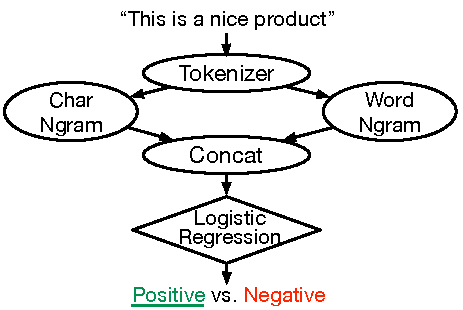
\includegraphics[width=0.36\textwidth]{dag-example.pdf}
    \caption{A Sentiment Analysis (SA) pipeline consisting of operators for featurization (ellipses), followed by a ML model (diamond). \emph{Tokenizer} extracts tokens (e.g., words) from the input string. \emph{Char} and \emph{Word Ngrams} featurize input tokens by extracting n-grams. \emph{Concat} generates a unique feature vector which is then scored by a \emph{Logistic Regression} predictor. This is a simplification: the actual DAG contains about 12 operators.}
    \label{fig:dag}
\end{wrapfigure}
%
\mlnet is an open-source C\# library running on a managed runtime with garbage collection and Just-In-Time (JIT) compilation~\footnote{Unmanaged C/C++ code can also be employed to speed up processing when possible.}.
\mlnet's main abstraction is called \idataview, which borrows ideas from the database community. Similarly to (intensional) database relations, the \idataview abstraction provides compositional processing of schematized data, but specializes it for ML pipelines. 
%
In relational databases, the term \emph{view} typically indicates the result of a query on one or more tables (base relations) or views, and is generally immutable~\cite{ views}.
Views have interesting properties that differentiate them from tables and make them appropriate abstractions for ML: (1) views are \emph{composable}---new views are formed by applying transformations (queries) over other views; (2) views are \emph{virtual}, i.e., they can be lazily computed on demand from other views or tables without having to materialize any partial results; and
(3) since a view does not contain values but merely computes values from its source views, it is \emph{immutable} and \emph{deterministic}: the exact same computation applied over the same input data always produces the same result.
Immutability and deterministic computation enables transparent data caching (for speeding up iterative computations such as ML algorithms) and safe parallel execution.
\idataview inherits the aforementioned database view properties, namely: composability, lazy evaluation, immutability, and deterministic execution.

In \mlnet, pipelines are represented as DAGs of operators, each of them implementing the \idataview interface and executing a featurization step or a ML model.
Upon pipeline initialization, the operators composing the model DAG are analyzed and arranged to form a chain of function calls which, at execution time, are JIT-compiled to form a unique function executing the whole DAG on a single call.
Operators are able to gracefully and efficiently handle high-dimensional and large datasets thanks to \emph{cursoring}, which resembles the well-known iterator model of databases~\cite{iterator-model}: 
within the execution chain, inputs are pulled through each operator to produce intermediate vectors that are input to the following operators, until a prediction or a trained model is rendered as the final output of the pipeline. We refer readers to~\cite{mldotnet2} for further details on \mlnet.


\section{Model Serving: An Overview}

\begin{figure}[!ht]
\vspace{-8ex}
   \subfigure[Models are deployed into containers, connected to a Serving System via RPC. To score the models, applications must call into the Web Server hosted on the Serving System using a REST API.]{
    \centering
        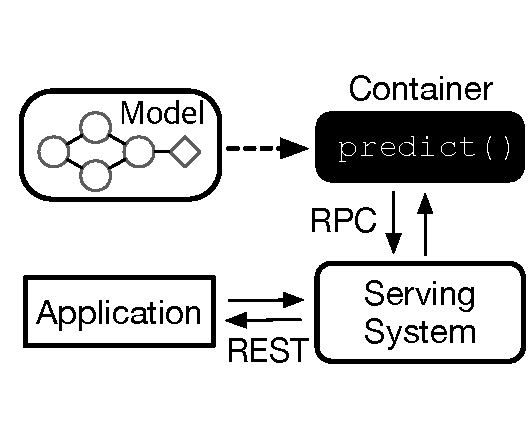
\includegraphics[width=0.32\textwidth]{container.pdf}
   }
   \hfill
   \subfigure[\mlnet allows developers to deploy models directly into their applications and without any additional custom engineering effort.]{
   \centering
        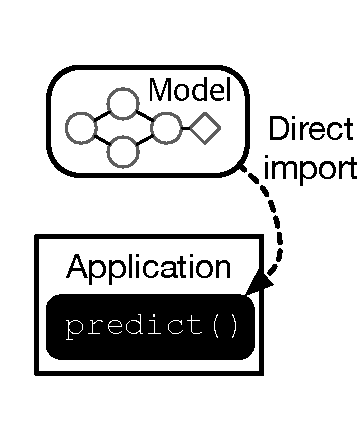
\includegraphics[width=0.21\textwidth]{application.pdf}
   }
   \hfill
   \subfigure[With the white-box approach, models' structural information can be used to optimize the execution. As in (b), applications can directly access the models by importing the Scoring Server Runtime.]{
   \centering
        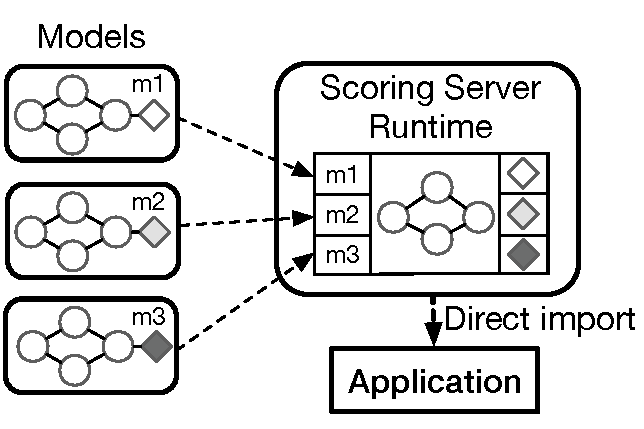
\includegraphics[width=0.36\textwidth]{white-box.pdf}
   }
   \caption{Three different ways to deploy models into applications. (a) and (b) represent two variations of the black-box approach where the invocation of the function chain (e.g., \texttt{predict()}) on a pipeline returns the result of the prediction. (c) shows the white-box approach.}
   \label{fig:existing-systems}
\end{figure}

In this Section, we survey how models are commonly operationalized in industry. 
The most popular (and easiest) method to deploy ML models (in general, and pipelines in particular) is what we refer to as \emph{black box}. 
Under this approach, internal pipelines' information and structures are not considered inasmuch as pipelines are opaque executable code accepting some input record(s) and producing a prediction.
%Figures~\ref{fig:existing-systems}(a) and ~\ref{fig:existing-systems}(b) depict two different flavours of how black box models are deployed. 
%The invocation of the function chain (e.g., \texttt{predict()}) on a pipeline returns the result of the prediction. 
Within the black box approach, there are two possible ways for a developer to deploy models, and consequently for an application to request and consume predictions.
The first option (\`a la Clipper~\cite{clipper}, depicted in Figure~\ref{fig:existing-systems}(a) and further described in Section~\ref{sec:clipper}) is to ship models into containers (e.g., Docker~\cite{docker}) wired with proper Remote Procedure Calls (RPCs) to a Web Server.
With this approach, predictions have to go through the network and be rendered on the cloud: low latency or edge scenarios are therefore out of scope.
The second option (Figure~\ref{fig:existing-systems}(b) and detailed in Section~\ref{sec:mlnet}) is to integrate the model logic directly into the application (\`a la \mlnet: the model is a dynamic library the application can link).
This approach is suitable for the cloud as well as for edge devices and it unlocks low latency scenarios. 
However, we still find this approach sub-optimal with respect to customized solutions because it ships the same training pipeline code for prediction. In fact, while using the same code is a great advantage because it removes the need for costly translation work, it implicitly assumes that training and prediction happen in the same regime. However, prediction serving is much more latency sensitive.
The \emph{white box} approach (Section~\ref{sec:white-box}) depicted in Figure~\ref{fig:existing-systems}(c) tackles the aforementioned problem by considering ML pipelines not anymore as black-box artifacts, but as DAGs of operators, and therefore it tries to rewrite them using optimizations specifically tailored to prediction-time scenarios.
We next provide additional details on each of the three possibilities. 

\subsection{Deploying Models into Containers}
\label{sec:clipper}

Most serving systems in the state of the art~\cite{clipper, msftmlserver, mms, tf-serving, clipper-nsdi, tf-serving2} aim to minimize the burden of deploying trained pipelines in production by serving them in containers, where the same code is used for both training and inference \footnote{Note that TensorFlow Serving~\cite{tf-serving} is slightly more flexible since users are allowed to split model pipelines and serve them into different containers (called \emph{servables}). However, this process is manual and occurs when building the container image, ignoring the final running environment.}.
This design allows decoupling models from serving system development, and eases the implementation of mechanisms and policies for fault tolerance and scalability.
Furthermore, hardware acceleration can be exploited when available.
A typical container-based, model serving system follows the design depicted in Figure~\ref{fig:existing-systems}(a): containers are connected to a Serving System (e.g., Clipper) via RPC, and, to score models, applications should contact the Serving System by invoking a Web Server through a REST API. Developers are responsible for setting up the communication between their applications and the Serving System, but this is in general an easy task as most Serving Systems provide convenient libraries (e.g., Microsoft ML Server~\cite{msftmlserver}).
Implementing model containers for new ML frameworks and integrating them with the Serving System requires a reasonable amount of effort: for example, a graduate student spent a couple of weeks to implement the protocol for integrating an \mlnet container into Clipper.  

\stitle{Limitations.}
While serving models via containers greatly eases operationalization, we found though that it is not flexible enough to accommodate the requirements stemming from running ML models at Microsoft scale. 
For instance, containers allow resource isolation and thus achieve effective multitenancy, but each container comes with its own runtime (e.g., an \mlnet instance) and set of processes, thus introducing memory overheads that can possibly be higher than the actual model size.
Additionally, the RPC layer and REST API introduce network communication costs, which are especially relevant for models that have millisecond-level prediction latency.
Finally, only a restricted set of optimizations are available, specifically those that do not require any knowledge of the internals of the pipelines; examples are handling multiple requests in batches and caching prediction results if some inputs queries are frequently issued for the same pipeline.
Instead, any optimization specific to the model is out of scope, as from the inscrutable nature of its container~\footnote{In the case of \mlnet pipelines, the C\# runtime in the container can optimize \emph{the code} of the model, but not the model itself as we propose in the following.}.
 
 \eat{
\begin{itemize}
    
    %\item Most of the state-of-the-art serving systems~\cite{tf-serving,tf-serving2, clipper, clipper-nsdi} aim to minimize the overhead of deploying trained pipelines in production by serving them into containers, where the same code is used for both training and inference.~\footnote{Note that TensorFlow Serving~\cite{tf-serving} is slightly more flexible since users are allowed to split model pipelines and serve them into different containers (called \emph{servables}). However this process is manual and not automatic.}
    
    %\item As shown in Figure~\ref{fig:existing-systems}(a), the containers are connected to the Serving System (e.g., Clipper) via RPC, which can be frequently done by different system engineers. To score the models, applications must contact the Serving System by invoking RESTful APIs. Application developers are responsible for setting up the communication between their applications and the Serving System. Moreover, implementing model containers and integrating them with the Serving System often requires non-trivial effort.
    
    \item \stitle{Limitations.}  
      \begin{itemize}
        \item \stitle{Waste of Space:} The container resources are isolated from each other, disallowing any part of models to be shared across different models. Deploying containers also causes memory overheads in order to maintain one separate runtime per container.
        
        \item \stitle{Network Communication Overhead:} The RPC layer and RESTful API introduce the cost for network communication, which consists of data transfer overhead, system calls invocation and serialization/de-serialization cost.
        
        \item \stitle{Coarse Grained Scheduling:} Under the black box approach: (1) a thread pool is used to serve multiple concurrent requests to the same model pipeline; (2) for each request, one thread handles the execution of a full pipeline sequentially~\footnote{Certain pipelines allow multi-threaded execution, but here we evaluate only single-threaded ones to estimate the per-thread efficiency.}, where one operator is active at each point in time; (3) shared operators/parameters are instantiated and evaluated multiple times (one per container) independently; (4) thread allocation is managed by the OS; and (5) load balancing is achieved ``externally'' by replicating containers when performance degradation is observed. We found this design sub-optimal, especially in heavily skewed scenarios where a small amount of popular models are scored more frequently than others.
        
        \item \stitle{Limited Optimizations:} Optimizations that can be applied are restricted to those that do not require the knowledge of the internals of the models (so called \emph{external} optimizations), such as handling multiple requests in batches and caching the results of the inference if some inputs queries are frequently issued for the same pipeline. Even though the models have a structure that can be optimized, the black box approach is not able to access such information and fails to optimize them.
    \end{itemize}
\end{itemize}
}

\subsection{Importing Models Directly into Applications}
\label{sec:mlnet}

At \msft, we have encountered the problem of model deployment across a wide spectrum of applications ranging from Bing Ads to Excel, PowerPoint and Windows 10, and running over diverse hardware configurations ranging from desktops, to custom hardware (e.g., XBox and IoT devices) and to high performance servers~\cite{windows-ai-platform, bing-ads, xbox}.
To allow such diverse use cases, an ML toolkit deeply embedded into applications should not only satisfy several intrinsic constraints (e.g., scale up or down based on the available main memory and number of cores) but also preserve the benefits commonly associated with model containerization, i.e., (1) it has to capture the full prediction pipeline that takes a test example from a given domain (e.g., an email with headers and body) and to produce a prediction that can often be structured and domain-specific (e.g., a collection of likely short responses); and (2) it has to allow to seamlessly carry the complete train-time pipeline into production for model inference.
This later requirement is the keystone for building effective, reproducible pipelines~\cite{google-rules-of-ml}.

\mlnet is able to implement all the above desiderata.
Once a model is trained in \mlnet, the full training pipeline can be saved and directly surfaced for prediction serving without any external modification.
Figure~\ref{fig:existing-systems}(b) depicts the \mlnet solution for black-box model deployment and serving: models are integrated into application logic natively and predictions can be served in any OS (Linux, Windows, Android, MacOS) or device supported by the .NET Core framework.
This approach removes the overhead of managing containers and implementing RPC functionalities to communicate with the Serving System. 
In this way, application developers are facilitated for writing applications with ML models inside. 
Nevertheless, models can still be deployed in the cloud if suggested by the application domain (e.g., because of special hardware requirements).

%\begin{itemize}
    %\item \mlnet, on the other hand, provides a way to integrate model code in the application logic more natively, which removes the overhead of managing container and implementing RPC protocol to communictate the serving system. This way, application developers can more easily write applications with ML model inside.
    
    %\item At \msft we have encountered this phenomenon across a wide spectrum of applications ranging from Bing Ads to Excel, Power Point and Windows 10, and running over diverse hardware configurations ranging from desktops to custom hardware (e.g., XBox and IoT devices) and high performance servers. A machine learning toolkit deeply embedded into applications, and allowing such diverse use cases must not only satisfy several intrinsic constraints (e.g., scale up or down based on the available main memory and number of cores) but also preserve the benefits commonly associated with model containerization, i.e., (1) it has to capture the full prediction pipeline that takes a test example from a given domain (e.g., an email with headers and body) and produces a prediction that can often be structured and domain-specific (e.g., a collection of likely short responses); and (2) it has to allow to seamlessly carry the complete train-time pipeline into production for model inference.
    %This later requirement is the keystone for building effective, reproducible pipelines~\cite{google-rules-of-ml}. 
    
    %\item Finally, serving the model for prediction is achieved by calling the \texttt{Predict} method with a list of training data objects.  Predictions can be served natively in any OS (e.g., Linux, Windows, Android, macOS) or device (x86/x64 and ARM processors) supported by the .NET Core framework.
%\end{itemize}
    
\stitle{Limitations.} \mlnet assumes no knowledge and no control over the pipeline inasmuch as the same code is executed both for training and prediction.~\footnote{Indeed, already trained operators will bypass the execution of the learning algorithm and directly apply the previously learned parameters.}
This is in general good practice because it simplifies the process of training-inference skew debugging~\cite{google-rules-of-ml}.
Nevertheless, we found that such approach is sub-optimal from a performance perspective.
For instance, transfer learning, A/B testing and model personalization are getting popular. Such trends produce models DAGs with high chance of overlapping structure and similar parameters, but these similarities cannot be recognized nor exploited using a black-box approach.
Furthermore, it is common practice for in-memory data-intensive systems to pipeline operators in order to minimize memory accesses for memory-intensive workloads, and to vectorize compute-intensive operators in order to minimize the number of instructions per data item~\cite{tupleware,journals/debu/ZukowskiBNH05}. \mlnet's operator-at-a-time model~\cite{journals/debu/ZukowskiBNH05} is sub-optimal because computation is organized around logical operators, ignoring how those operators behave together: in the example of the sentiment analysis pipeline of Figure~\ref{fig:dag}, logistic regression is commutative and associative (e.g., dot product between vectors) and can be pipelined with Char and WordNgram, eliminating the need for the Concat operation and the related buffers for intermediate results.
Note that this optimization is applicable only at prediction-time whereas at training-time logistic regression runs the selected optimization algorithm.
We refer readers to~\cite{pretzel-osdi} for further limitations arising when serving models for prediction using the black-box approach.
   

% \subsection{Limitations}
% To optimize the performance, the black box systems including \mlnet apply techniques such as handling multiple requests in batches and caching the results of the inference if some predictions are frequently issued for the same pipeline. 
% However, these techniques assume no knowledge and no control over the pipeline, and are unaware of its internal structure.
% Despite being regarded as a good practice~\cite{google-rules-of-ml}, the black box, this design hides the structure of each served model and prevents the system from controlling and optimizing the pipeline execution. 
% %Therefore, under this approach, there is no principled way neither for sharing optimizations between pipelines, nor to improve the end-to-end execution of individual pipelines.
% We observed the following limitations in current state-of-the-art prediction serving systems.\ys{short description for each limitation. Memory waste is deferred to the next section, where we talk about cloud}
% \begin{itemize}
%     \item Non-uniform Accesses
%     \item Coarse Grained Scheduling
%     \item Operator-at-a-time Model
%     \item Prediction Initialization
% \end{itemize}


% ML is usually conceptualized as a two-steps process: first, during \emph{training} model parameters are estimated from large datasets by running computationally intensive iterative algorithms; successively, trained pipelines are used for \emph{inference} to generate predictions through the estimated model parameters.
% When trained pipelines are served for inference, the full set of operators is deployed altogether to massage and featurize the raw input data before ML model prediction rendering.
% However, pipelines have different system characteristics based on the phase in which they are employed: for instance, at training time ML models run complex algorithms to scale over large datasets (e.g., linear models can use gradient descent in one of its many flavors~\cite{DBLP:journals/corr/Ruder16,NIPS2011_4390,sdca}), while, once trained, they behave as other regular featurizers and data transformations; furthermore, during inference pipelines are often surfaced for direct users' servicing and therefore require low latency, high throughput, and graceful degradation of performance in case of load spikes.\ys{Explain \pretzel recognize the model serving and the training to be different, and optimize the serving considering these aspects.}


\subsection{White Box Model Serving}
\label{sec:white-box}
As we have seen so far, black-box approaches disallow any optimization and sharing of resources among models. 
Such limitations are overcome by the \emph{white box approach} embraced by systems such as TVM~\cite{tvm} and \pretzel~\cite{pretzel-osdi}. 
%White box system allows the optimization of predictions both horizontally \emph{end-to-end} and vertically \emph{among multiple model pipelines}.
Figure~\ref{fig:existing-systems}(c) sketches white-box prediction serving. Models are registered to a Runtime that considers them not as mere executable code but as DAGs of operators. 
Applications can request predictions by directly including the Runtime in their logic (similarly to how SQLite databases~\cite{sqlite} can be integrated into applications), or by submitting a REST request to a cloud-hosted Runtime.
The white box approach enables the Runtime to apply optimizations over the models such as operator reordering to improve latency or operator and sub-graph sharing to improve memory consumption and computation reuse (through caching).
Thorough scheduling of pipelines' components can be managed within the Runtime, which controls the whole workload so that optimal allocation decisions can be made for running machines to high utilization and avoid many of the aforementioned overheads.
In general, we have identified the following optimization opportunities for white-box model serving.

\stitle{End-to-end Optimizations:} The operationalization of models for prediction should focus on computation units making optimal decisions on how data are processed and results are computed, to keep low latency and graceful degradation of performance with increasing load. Such computation units should: (1) avoid memory allocation on the data path; (2) avoid creating separate routines per operator when possible, which are sensitive to branch mis-prediction and poor data locality~\cite{Neumann:2011:ECE:2002938.2002940}; and (3) avoid reflection and JIT compilation at prediction time. Optimal computation units can be compiled Ahead-Of-Time (AOT) since pipeline and operator characteristics are known upfront, and often statistics from training are available. The only decision to make at runtime is where to allocate the computation units based on available resources and constraints.

\stitle{Multi-model Optimizations:} To take full advantage of the fact that pipelines often use similar operators and parameters, shareable components have to be uniquely stored in memory and reused as much as possible to achieve optimal memory usage. Similarly, execution units should be shared at runtime and resources should be properly pooled and managed, so that multiple prediction requests can be evaluated concurrently. 
Partial results, for example outputs of featurization steps, can be saved and re-used among multiple similar pipelines.

Out of these guidelines, the next Section describes a prototype runtime for \mlnet enabling white-box model serving.

% \section{Towards Model Serving in the Cloud}
% \mi{I don't think we need this anymore. Maybe we can move it later to say that for the moment we have tested our database runtime in the cloud.}
% \begin{itemize}
%     % \pretzel#Sec2
%     \item Nowadays, ``intelligent'' services such as Microsoft Cortana speech recognition, Netflix movie recommender or Gmail spam detector depend on ML scoring capabilities, which are currently experiencing a growing demand~\cite{Crankshaw:2018:PS:3194653.3210557}. This in turn fosters the research in prediction serving systems in cloud settings~\cite{tf-serving,tf-serving2,clipper,clipper-nsdi}, where trained models are operationalized in the cloud environment.
%     \item In the cloud, systems need to consider another performance metric; to increase the density of models in machines. In particular, ML service providers tend to run many models concurrently while hosting ML-based services. As running more models, the amount of resources increases and thus the operational cost also increases. 
%     \item More interesingly, many models have the common structures due to the recent trends of personalization, fine tuning, transfer learning.
%     \item The aforementioned \emph{black box} approaches bring additional challenges; models are not allowed to share common part, which leads to resources (specifically memory) to be wasted. In addition, CPU resources can be wasted if many models are served concurrently, as the model containers use the CPU resources without coordination.
% \end{itemize}

\section{A Database Runtime for Model Serving}
    
Following the guidelines of white-box model serving, we implemented \pretzel~\cite{pretzel-osdi,iccd}, a new runtime for \mlnet specifically tailored for high-performance prediction serving.
\pretzel views models as data\-base queries and employs database techniques to optimize DAGs and to improve end-to-end performance. The problem of optimizing co-located pipelines is casted as a multi-query optimization and techniques such as view materialization are employed to speed up pipeline execution. Memory and CPU resources are shared in the form of vector and thread pools, such that overheads for instantiating memory and threads are paid only upfront at initialization time.
\pretzel is organized in 6 main components. A \emph{data-flow-style language integrated API} called \at{Flour} with related \emph{compiler} and \emph{optimizer} called \at{Oven} are used in concert to convert \mlnet pipelines into \emph{model plans}. An \at{Object} \at{Store} saves and shares parameters among plans. A \at{Runtime} manages compiled plans and their execution, while a \at{Scheduler} manages the dynamic decisions on how to schedule plans based on machine workload. Finally, a \at{FrontEnd} is used to submit prediction requests to the system. 

In \pretzel, deployment and serving of model pipelines follow a two-phase process as illustrated in Figure~\ref{fig:white-box}(a) and~\ref{fig:white-box}(b). 
%where the \emph{off-line phase} is done completely in advance, and the \emph{on-line phase} is executed at inference time.
During the \emph{off-line phase}, pre-trained \mlnet pipelines are translated into \at{Flour} transformations. \at{Oven} optimizer re-arranges and fuses transformations into model plans composed of parameterized logical units called \emph{stages}. Each logical stage is then AOT-compiled into physical computation units.
Logical and physical stages together with model parameters and training statistics form a model plan. %where memory resources and threads are pooled at runtime. 
Model plans are registered for prediction serving in the \at{Runtime} where physical stages and parameters are shared among pipelines with similar model plans. In the \emph{on-line phase}, when an inference request for a registered model plan is received, physical stages are parameterized dynamically with the proper values maintained in the \at{Object} \at{Store}. The \at{Scheduler} is in charge of binding physical stages to shared execution units.

\begin{figure}[!ht]
   \subfigure[Model optimization and compilation in \pretzel: (1) A model is translated into a \at{Flour} program. (2) \at{Oven} \at{ Optimizer} generates a DAG of logical stages from the program. Additionally, parameters and statistics are extracted. (3) A DAG of physical stages is generated by the \at{Oven} \at{Compiler} using logical stages, parameters, and statistics. A model plan is the union of all the elements.\label{fig:system-design-offline}]{
        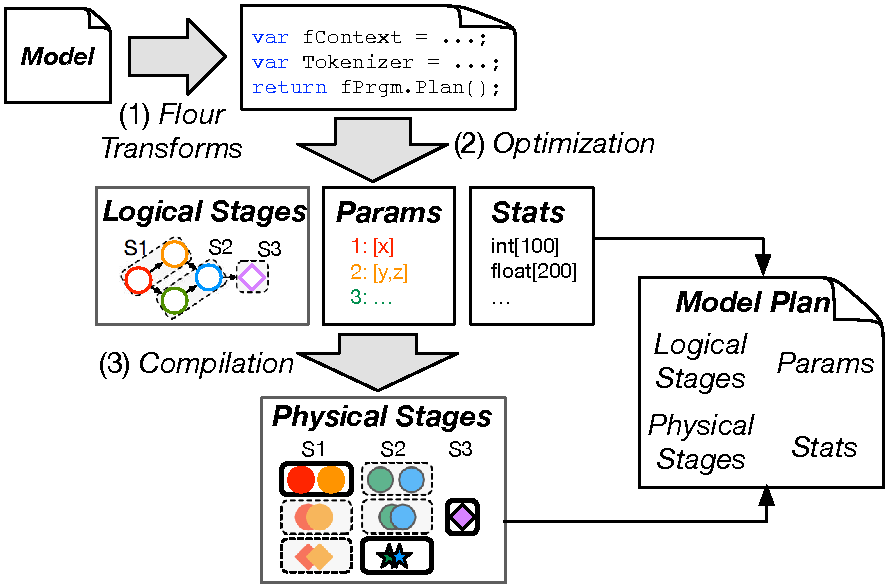
\includegraphics[width=0.48\textwidth]{offline.pdf}
   }
   \hfill
   \subfigure[(1) When a prediction request is issued, (2) the \at{Runtime} determines  whether to serve the prediction using (3) the request/response engine or (4) the batch engine. In the latter case, the \at{Scheduler} takes care of properly allocating stages over the Executors running concurrently on CPU cores. (5) The \at{FrontEnd} returns the result to the Client once all stages are complete.\label{fig:system-design-online}]{
        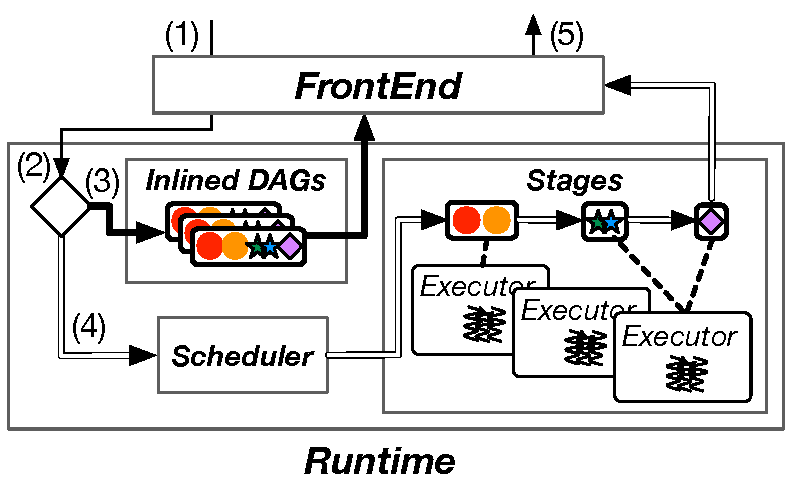
\includegraphics[width=0.46\textwidth]{online.pdf}
   }
   \caption{How \pretzel system works in two phases: (a) Offline and (b) Online.}
   \label{fig:white-box}
\end{figure}

\pretzel compiles a model pipeline into an optimized, executable plan following 3 steps:

\begin{enumerate}
    \item \stitle{Model conversion:} \at{Flour} is an an intermediate representation, which makes \pretzel's optimizations applicable to various ML frameworks (although the currently implementation is for ML.NET). Once a pipeline is ported into \at{Flour}, it can be optimized and compiled into a model plan. \at{Flour} provides a language-integrated API similar to KeystoneML~\cite{keystone-ml} or LINQ~\cite{linq}, where sequences of transformations are chained into DAGs and lazily compiled for execution.

    \item \stitle{Optimization:} \at{Oven}'s rule-based Optimizer rewrites a model pipeline represented in \at{Flour} into a graph of logical stages. 
    Initially, the Optimizer applies rules for schema propagation, schema validation and graph validation. The rules check whether the input schema of each data transformation is valid (e.g., WordNgram in Figure 1 takes a text as input) and the structure of the graph is well-formed (e.g., only one final predictor model at the end). The next rules are used to build stages by traversing the entire graph to find \emph{pipeline-breaking} transformations that require all inputs to be fully materialized (e.g., normalizer): all transformations up to that point are then grouped into a stage.
    By leveraging stage graphs similar to Spark~\cite{rdd-nsdi2012}, \pretzel can run computations more efficiently than the operator-at-a-time strategy of \mlnet. The stage graph is then optimized by recursively applying rules such as (1) removing unnecessary branches (similar to common sub-expression elimination); (2) merging stages containing identical transformations; (3) inlining stages that contain only one transformation.
    
    \item \stitle{Compilation:} After building the stage graph, a \emph{Model Plan Compiler} (MPC) translates the graphs into physical stages, which are AOT-compiled, parameterized, and result in lock-free computation unit. Logical and physical stages have a 1-to-n mapping, and MPC selects the most efficient physical implementation given the logical stage's parameters (e.g., the maximum length of n-grams) and statistics (e.g., whether the vector is dense or sparse). During the translation process, MPC saves the additional parameters required for running stage code (e.g., a dictionary consisting of frequency of n-grams) into the \at{ObjectStore} in order to share them with other stages with the same parameters. 
    Finally, model plans are registered into the \at{Runtime}. Model plans consist of mappings between logical representations, physical implementations and the associated parameters. Upon registration, physical stages composing a plan are loaded into a system catalog. When a prediction request is submitted to the system, the AOT-compiled physical stages are initialized with the parameters from the mapping in the model plan, which allows \pretzel \at{Runtime} to share the same physical implementation among multiple pipelines.
\end{enumerate}

\section{Conclusion}

% \stitle{Off-line Phase:}
% \pretzel has two limitations regarding \at{Flour} and \at{Oven} design. First, \pretzel currently has several logical and physical stages classes, one per possible implementation, which make the system difficult to maintain in the long run. 
% Additionally, different back-ends (e.g., \pretzel currently supports operators implemented in C\# and C++, and experimentally on FPGA~\cite{iccd}) require all specific operator implementations. We are however confident that this limitation will be overcome once code generation of stages will be added (e.g., with hardware-specific templates~\cite{conf/icde/KrikellasVC10}).
% Secondly, \at{Flour} and \at{Oven} are currently limited to pipelines authored in \mlnet, and porting models from different frameworks to the white box approach may require non-trivial work.
% On the long run our goal is, however, to target unified formats such as ONNX~\cite{onnx}; this will allow us to apply the discussed techniques to models from other ML frameworks as well.

% \stitle{On-line Phase:}
% \pretzel's fine-grained, stage-based scheduling may introduce additional overheads in contrasts to coarse-grained whole pipeline scheduling due to additional buffering and context switching. However, such overheads are related to the system load and therefore controllable by the scheduler.
% Additionally, we found GC overheads to introduce spikes in latency. Although our implementation tries to minimize the number of objects created at runtime, in practice we found that long tail latencies are common.
% On white box architectures, failures happening during the execution of a model may jeopardize the whole system. We are currently working on isolating model failures over the target Executor. 
% Finally, \pretzel runtime currently runs on a single-node. An experimental scheduler adds Non Uniform Memory Access (NUMA) awareness to scheduling policies. We expect this scheduler to bring benefits for models served from large instances (e.g., \cite{numa-aws}). 
% We expect in the future to be able to scale the approach over distributed machines, with automatic scale in/out capabilities.


Inspired by the growth of ML applications and ML-as-a-service platforms, this paper identifies three strategies for operationalizing trained models: container-based, direct import into applications, and the white-box approach.
Using \mlnet as use case, we listed a set of limitations on how existing systems fall short in key requirements for ML prediction-serving, disregarding the optimization of model execution in favor of ease of deployment. 
Finally, we describe how the problem of serving predictions can be casted as a database problem, whereby end-to-end and multi-query optimization strategies are applied to ML pipelines.

We recognize that much work remains to be done for achieving a seamless and efficient integration of ML models with applications and development processes. 
While we believe that \mlnet and \pretzel are a step in the right direction, equivalents in data science for common tools and techniques in software development (e.g., unit/integration test, build server, code review, versioning, backward compatibility, and lifecycle management) are not defined yet. 
We encourage the community to engage in the work towards closing those gaps.
%To decrease latency, we have developed an optimizer and compiler framework generating efficient model plans end-to-end. 
%To decrease the memory footprint and increase resource utilization and throughput, we allow pipelines to share parameters and physical operators, and defer the problem of inference execution to a scheduler that allows running multiple predictions concurrently on shared resources.

%Experiments with production-like pipelines show the validity of our approach in achieving an optimized execution: \pretzel delivers order-of-magnitude improvements on previous approaches and over different performance metrics. 


\itemsep=1pt 
\begin{small}
\begin{thebibliography}{10}

\bibitem{windows-ai-platform}
AI Platform for Windows Developers.
\newblock \url{https://blogs.windows.com/buildingapps/2018/03/07/ai-platform-windows-developers}

\bibitem{mllib}
Apache Spark MLlib.
\newblock \url{https://spark.apache.org/mllib}

\bibitem{clipper}
{Clipper.}
\newblock \url{http://clipper.ai}

\bibitem{docker}
Docker.
\newblock \url{https://docker.com}

\bibitem{bing-ads}
The future of AI marketing: human ingenuity amplified.
\newblock \url{https://advertise.bingads.microsoft.com/en-us/insights/g/artificial-intelligence-for-marketing}

\bibitem{h2o}
H2O.ai.
\newblock \url{https://www.h2o.ai}

\bibitem{xbox}
Microsoft Looks To Patent AI For Detecting Video Game Cheaters.
\newblock \url{https://www.cbinsights.com/research/microsoft-xbox-machine-learning-cheat-detection-gaming-patent}

\bibitem{msftmlserver}
{Microsoft Machine Learning Server}.
\newblock
\url{https://docs.microsoft.com/en-us/machine-learning-server}

\bibitem{mldotnet}
{{ML.N}et}.
\newblock
 \url{https://dot.net/ml}

\bibitem{mms}
{MXN}et {M}odel {S}erver ({MMS}).
\newblock \url{https://github.com/awslabs/mxnet-model-server}

\bibitem{sqlite}
SQLite.
\newblock \url{https://www.sqlite.org}

\bibitem{tf-serving}
{Tensor{F}low Serving.}
\newblock \url{https://www.tensorflow.org/serving}

\bibitem{mldotnet2}
Z.~Ahmed, and et al.
\newblock Machine Learning for Applications, not Containers.
\newblock {\em Under Submission}, 2018.

\bibitem{tvm}
T.~Chen, T.~Moreau, Z.~Jiang, L.~Zheng, E.~Yan, H.~Shen, M.~Cowan, L.~Wang, Y.~Hu, L.~Ceze, C.~Guestrin, and A.~Krishnamurthy.
\newblock {{TVM}: An Automated End-to-End Optimizing Compiler for Deep Learning}.
\newblock {\em OSDI}, 2018

\bibitem{clipper-nsdi}
D.~Crankshaw, X.~Wang, G.~Zhou, M.~J.~Franklin, J.~E.~Gonzalez, and I.~Stoica.
\newblock Clipper: {A} Low-Latency Online Prediction Serving System.
\newblock {\em NSDI}, 2017.

\bibitem{tupleware}
A.~Crotty, A.~Galakatos, K.~Dursun, T.~Kraska, C.~Binnig, U.~Cetintemel, and S.~Zdonik.
\newblock An Architecture for Compiling {UDF}-centric Workflows.
\newblock {\em VLDB}, 2015.

\bibitem{iterator-model}
G.~Graefe.
\newblock {Volcano: An Extensible and Parallel Query Evaluation System.}
\newblock {\em IEEE Trans. on Knowl. and Data Eng.}, {February 1994}.

\bibitem{views}
{A.~Y.~Halevy}
\newblock {Answering Queries Using Views: A Survey.}
\newblock {\em VLDB Journal}, December 2001.

\bibitem{pretzel-osdi}
Y.~Lee, A.~Scolari, B.~-G.~Chun, M.~D.~Santambrogio, M.~Weimer, and M. Interlandi.
\newblock \pretzel: Opening the black box of Machine Learning Prediction Serving.
\newblock {\em OSDI}, 2018.

\bibitem{linq}
{E.~Meijer, B.~Beckman, and G.~Bierman}
\newblock {{LINQ}: Reconciling Object, Relations and {XML} in the {.NET} Framework}.
\newblock {\em SIGMOD}, 2006.

\bibitem{Neumann:2011:ECE:2002938.2002940}
T.~Neumann.
\newblock {Efficiently Compiling Efficient Query Plans for Modern Hardware.}
\newblock {\em VLDB Endowment}, June 2011.

\bibitem{tf-serving2}
C.~Olston, F.~Li, J.~Harmsen, J.~Soyke, K.~Gorovoy, L.~Lao, N.~Fiedel, S.~Ramesh, and V.~Rajashekhar.
\newblock {TensorFlow-Serving: Flexible, High-Performance ML Serving.}
\newblock {\em Workshop on ML Systems at {NIPS}}, 2017.

\bibitem{scikit}
F.~Pedregosa, G.~Varoquaux, A.~Gramfort, V.~Michel, B.~Thirion, O.~Grisel, M.~Blondel, P.~Prettenhofer, R.~Weiss, V.~Dubourg, J.~Vanderplas, A.~Passos, D.~Cournapeau, M.~Brucher, M.~Perrot, and \'{E}.~Duchesnay.
\newblock Scikit-learn: Machine Learning in Python.
\newblock {\em J. Mach. Learn. Res.}, 2011.

\bibitem{iccd}
A.~Scolari, Y.~Lee, M.~Weimer, and M. Interlandi.
\newblock Towards Accelerating Generic Machine Learning Prediction Pipelines.
\newblock {\em {IEEE} ICCD}, 2017.

\bibitem{keystone-ml}
{E.~R.~Sparks, S.~Venkataraman, T.~Kaftan, M.~J.~Franklin, and B.~Recht}.
\newblock {Keystone{ML}: Optimizing Pipelines for Large-Scale Advanced Analytics}.
\newblock {\em ICDE}, 2017

\bibitem{rdd-nsdi2012}
M.~Zaharia, M.~Chowdhury, T.~Das, A.~Dave, J.~Ma, M.~McCauley, M.~J.~Franklin, S.~Shenker, and I.~Stoica.
\newblock {{R}esilient {D}istributed {D}atasets: A Fault-Tolerant Abstraction for In-Memory Cluster Computing}.
\newblock {\em NSDI}, 2012

\bibitem{google-rules-of-ml}
M.~Zinkevich.
\newblock Rules of Machine Learning: Best Practices for {ML} Engineering.
\newblock \url{https://developers.google.com/machine-learning/rules-of-ml}

\bibitem{journals/debu/ZukowskiBNH05}
M.~Zukowski, P.~A.~Boncz, N.~Nes, and S.~H\'{e}man.
\newblock {Monet{DB/X}100 - A {DBMS} in the {CPU} Cache.}
\newblock {\em IEEE Data Eng. Bull.}, 2005.


% \bibitem{onnx}
% Open {N}eural {N}etwork {E}xchange ({ONNX}).
% \newblock \url{https://onnx.ai}

% \bibitem{keras}
% {Keras.}
% \newblock \url{https://www.tensorflow.org/api_docs/python/tf/keras}

% \bibitem{tensorflow}
% Tensor{F}low.
% \newblock \url{https://www.tensorflow.org}

% \bibitem{caffe2}
% Caffe2.
% \newblock \url{https://caffe2.ai}

% \bibitem{numa-aws}
% EC2 large instances and NUMA.
% \newblock \url{https://forums.aws.amazon.com/thread.jspa?threadID=144982}

% \bibitem{DBLP:journals/corr/Ruder16}
% Ruder, Sebastian.
% \newblock {An overview of gradient descent optimization algorithms.}
% \newblock In CoRR, 2016.

% \bibitem{NIPS2011_4390}
% Recht, Benjamin and Re, Christopher and Wright, Stephen and Feng Niu.
% \newblock {Hogwild: A Lock-Free Approach to Parallelizing Stochastic Gradient Descent.}
% \newblock In NIPS, 2011.

% \bibitem{sdca}
% Shalev-Shwartz, Shai and Zhang, Tong
% \newblock {Stochastic Dual Coordinate Ascent Methods for Regularized Loss.}
% \newblock In J. Mach. Learn. Res., 2013

% \bibitem{Crankshaw:2018:PS:3194653.3210557}
% Crankshaw, Dan and Gonzalez, Joseph.
% \newblock Prediction-Serving Systems.
% \newblock In {{ACM Q}ueue}, 2018.

%\bibitem{conf/icde/KrikellasVC10}
%Krikellas, Konstantinos and Viglas, Stratis and Cintra, Marcelo.
%\newblock Generating code for holistic query evaluation.
%\newblock In ICDE, 2010.

\end{thebibliography}
\end{small}

\end{document}